%%%%%%%%%%%%%%%%%%%%%%%%%%%%%%%%%%%%%%%%%
% Short Three-Column Newsletter
% LaTeX Template
% Version 1.0 (11/9/13)
%
% Original author:
% Frits Wenneker (http://www.howtotex.com) 
% With extensive modifications by:
% Vel (vel@latextemplates.com)
% 
% This template has been downloaded from:
% http://www.LaTeXTemplates.com
%
% License:
% CC BY-NC-SA 3.0 (http://creativecommons.org/licenses/by-nc-sa/3.0/)
%
%%%%%%%%%%%%%%%%%%%%%%%%%%%%%%%%%%%%%%%%%

%----------------------------------------------------------------------------------------
%	PACKAGES AND DOCUMENT CONFIGURATIONS
%----------------------------------------------------------------------------------------

\documentclass[8pt,a4paper]{article} % Paper type (a4paper, usletter or legal) and font size (10, 11 or 12)
\usepackage{extsizes}
\setlength\topmargin{-48pt} % Top margin
\setlength\headheight{0pt} % Header height
\setlength\textwidth{7.0in} % Text width
\setlength\textheight{9.5in} % Text height
\setlength\oddsidemargin{-30pt} % Left margin
\setlength\evensidemargin{-30pt} % Left margin (even pages) - only relevant with 'twoside' article option

\usepackage{charter} % Charter font for main content

\frenchspacing % Reduces space after periods to make text more compact for a three-column layout
\usepackage[spanish]{babel}
\usepackage[utf8]{inputenc} % Caracteres con acentos. 
\usepackage[T1]{fontenc}%paquete principal3
\usepackage{graphicx} % Required for including images
\usepackage{amssymb,amsmath} % Math packages
\usepackage{multicol} % Required for the three-column layout of the document
\usepackage{url} % Clickable links
\usepackage{enumitem} % Reduces the amount of space within and between lists with [noitemsep,nolistsep]
\usepackage{marvosym} % Required for the use of symbols
\usepackage{wrapfig} % Allows wrapping text around figures
\usepackage[T1]{fontenc} % Use 8-bit encoding that has 256 glyphs
\usepackage{datetime} % Required for defining a custom date style
\newdateformat{mydate}{\monthname[\THEMONTH] \THEYEAR} % Set a custom date format
\usepackage[pdfpagemode=FullScreen, colorlinks=false]{hyperref} % Link colors and PDF behavior in Acrobat
\usepackage{fancyhdr} % Required to define custom headeadapatacionrs/footers
\pagestyle{fancy} % Enables the custom headers/footers for all pages following this

%-----------------------------------------------------------
% Header and footer
\lfoot{\footnotesize % Left footer containing newsletter contact information
CBPE/ISLP-BOLIVIA\\
* CBPE: Competencia Boliviana de Posters Estadísticos\\
** INE: Instituto Nacional de Estadística, entidad reconocida por el estado boliviano, para estadísticas estatales \\
\Mundus\ \href{https://islp-bolivia.github.io}{https://islp-bolivia.github.io} \quad
\Telefon\  (+591) 2004492 \quad
\Letter\ \href{mailto:islp.bolivia@gmail.com}{islp.bolivia@gmail.com}
}

\cfoot{} % Empty center footer

\rfoot{\footnotesize ~\\ Page \thepage} % Right footer - page counter

\renewcommand{\headrulewidth}{0.0pt} % No horizontal rule for the header
\renewcommand{\footrulewidth}{0.4pt} % Horizontal rule separating the footer from the document
%-----------------------------------------------------------

%-----------------------------------------------------------
% Define separators
\newcommand{\HorRule}[1]{\noindent\rule{\linewidth}{#1}} % Creates a horizontal rule
\newcommand{\SepRule}{\noindent	% Creates a shorter separator rule
\begin{center}
\rule{250pt}{1pt} % Page width and rule width
\end{center}
}
%-----------------------------------------------------------

%-----------------------------------------------------------
% Define title and article styles
\newcommand{\NewsletterName}[1]{ % Newsletter title
\begin{center}
\Huge \usefont{T1}{fvs}{b}{n} % Use the Bera Sans Bold font
#1
\end{center}	
\par \normalsize \normalfont}

\newcommand{\JournalIssue}[1]{ % Date and issue number at the top of the newsletter
\hfill \textsc{\mydate \today, No #1} % Right-aligned date and issue number
\par \normalsize \normalfont}

\newcommand{\NewsItem}[1]{ % News item title
\usefont{T1}{fvs}{n}{n} % Use the Bera Sans Normal font
\vspace{24pt}\large #1\vspace{3pt} % Print the title with space around it in a larger font size
\par \normalsize \normalfont}

\newcommand{\NewsAuthor}[1]{ % Author name under the item title
\hfill Por \textsc{#1} \vspace{20pt} % Right-aligned author name in small caps with space after it
\par \normalfont}		

%----------------------------------------------------------------------------------------
%	TITLE
%----------------------------------------------------------------------------------------

\begin{document}

\JournalIssue{1} % Issue number

\NewsletterName{Boletín Nro. 1\\ 
''Lanzamiento Oficial de la Competencia Boliviana de Posters Estadísticos''} % Newsletter title
\NewsAuthor{CBPE* / ISLP-BOLIVIA}
\noindent\HorRule{3pt} \\[-0.75\baselineskip] % Thick horizontal rule
\HorRule{1pt} % Thin horizontal rule

%----------------------------------------------------------------------------------------
%	MAIN NEWS ITEM
%----------------------------------------------------------------------------------------

%\setlength{\columnsep}{16pt} % Uncomment to manually change the white space between columns
\begin{multicols}{2} % Begin the three-column layout

%----------------------------------------------------------------------------------------
%	OTHER NEWS
%----------------------------------------------------------------------------------------
\NewsItem{\textbf{Avanzando hacia la Alfabetización Estadística!!!}} 

\vspace{0.2cm}

\begin{center}
\includegraphics[scale=0.14]{foto11.jpg} % Example of an in-line image
\end{center}

\vspace{0.2cm}

Con el propósito de promover acciones concretas para impulsar la alfabetización estadística en Bolivia, el Instituto Nacional de Estadística (INE) y la Fundación ARU en cooperación mutua, realizarón el lanzamiento
 oficial de la {\it ''Competencia Boliviana de Posters Estadísticos 2018-2019''}, por primera vez en Bolivia.\\
 
 En esta su primera versión la competencia pretende fomentar el uso, análisis, interpretación y comunicación de datos e
 información estadística, en jóvenes y adolescentes de todo el país.

\NewsItem{\textbf{Lanzamiento de la Competencia}} 

\vspace{0.2cm}

El evento de lanzamiento tuvo lugar
 el jueves 5 de julio de 2018,  en el auditorio ''Jorge Félix Ballivian'' del INE, en el evento también participaron
 representantes de las instituciones patrocinadoras de la Competencia, Banco Mundial, Organización de las 
Naciones Unidas para la Alimentación y la Agricultura (FAO), el Fondo de las Naciones Unidas para la Infancia (UNICEF),
 Carrera de Estadística - UMSA y Universidad Privada de Santa Cruz de la Sierra - UPSA, como también medios de comunicación.

\begin{center}
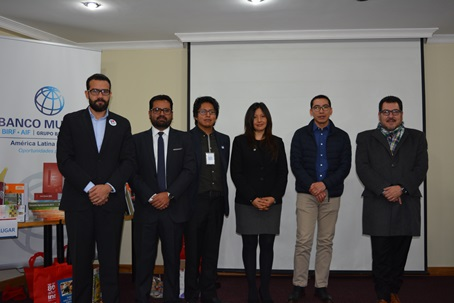
\includegraphics[scale=0.13]{foto2.jpg} % Example of an in-line image
\end{center}

%-----------------------------------------------------------
\NewsItem{\textbf{El valor de la  CBPE en las estadísticas bolivianas}}

\vspace{0.2cm}

\begin{center}
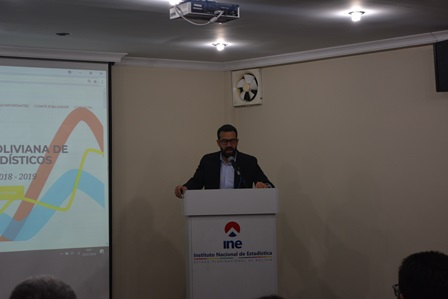
\includegraphics[scale=0.15]{foto3.jpg} % Example of an in-line image
\end{center}

\vspace{0.2cm}

{\tt Director General Ejecutivo del INE, Santiago Farjat Bascón}, \textit{''Celébro los esfuerzos conjuntos que realizamos para promover la cultura estadística en Bolivia y ayudar a las sociedades desde muy corta edad, a empaparse de lo que es la estadística'' . Los objetivos primordiales de este 
concurso, son fortalecer las capacidades para interpretar y evaluar críticamente la información estadística ''a la 
cual nos encontramos diariamente expuestos'' y mejorar las capacidades para la discusión, razonamiento estadístico y 
la comunicación comprensible de los datos.}\\

El INE** ha dispuesto para los ganadores de la competencia en sus diferentes categorías, 1.065
 publicaciones como premios: 

\begin{multicols}{2}
\begin{small}
\begin{itemize}
\item Series Históricas 80 años Generando Estadísticas, Censo de Población y Vivienda 2012, Censo Agropecuario 2013, Anuarios Estadísticos, publicaciones de las Encuestas de Hogares
\item Mochilas, juegos de mesa y memorias extraíbles.
\end{itemize}
\end{small}
\end{multicols}

\NewsItem{\textbf{Proceso de involucramiento}}

\begin{center}
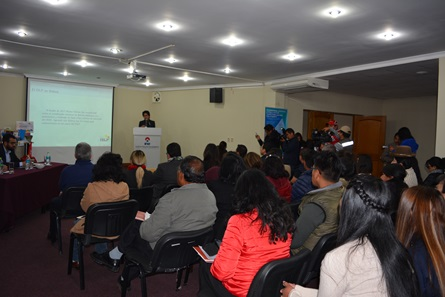
\includegraphics[scale=0.15]{foto4.jpg} % Example of an in-line image
\end{center}

Con la participación de instituciones estatales y entidades públicas que desarrollan estadísticas en Bolivia, más la participación de instituciones patrocinadoras de la competencia, se hace pública la invitación a estudiantes, adolescentes y jovenes de toda Bolivia a través de medios de comunicación, con la conferencia de prensa realizada después del evento inaugural. En el evento se dio a conocer la página de inscripción e información de la ''Competencia Boliviana de Posters Estadísticos''\url{https://islp-bolivia.github.io/}.


%--------------------------
\NewsItem{\textbf{Inscripciones abiertas}}

La ''Competencia Boliviana de Posters Estadísticos 2018-2019'', da la bienvenida al concurso, a sus diferentes participantes en las tres categorias abiertas: Bernoulli (Adolescentes nacidos en los años 2003, 2004 y 2005); Poisson (Adolescentes y jóvenes nacidos en los años 2000, 2001 y 2002) y Gauss (Estudiantes de pregrado de universidades públicas o privadas sin límite de edad), al finalizar la competencia se premiarán con paquetes estudiantiles y publicaciones del INE  al  primer, segundo y tercer lugar de cada categoría.

\vspace{0.5cm}

\begin{center}
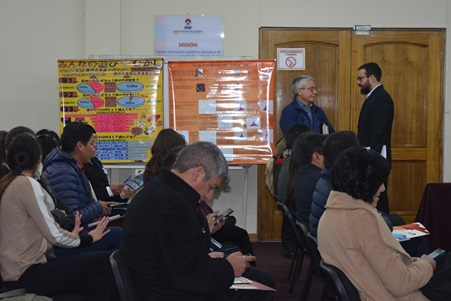
\includegraphics[scale=0.15]{foto6.jpg} % Example of an in-line image
\end{center}

\vspace{10cm}

\begin{center}
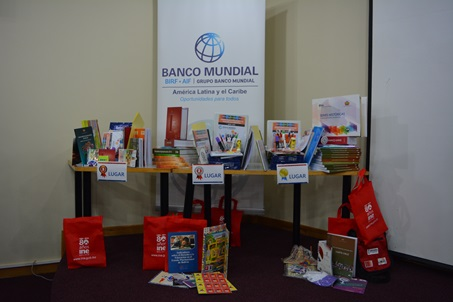
\includegraphics[scale=0.15]{foto5.jpg} % Example of an in-line image
\end{center}

\vspace{10cm}

\end{multicols} % End the three-column layout for a large picture
%----------------------------------------------------------------------------------------


\end{document} 